\label{sec:ablation}
Given the signal-validation result (Table~\ref{tab:signals}), we ran the
full ReAct$\to$CoT-SC hybrid ($n{=}100$/domain, $n_{sc}{=}5$) for two
arms: \texttt{paper} ($S_1$ only, control) and \texttt{s1s3}
($S_1 \lor S_3$). We did not scale up the $S_2$-containing composite arms
(\texttt{s1s2}, \texttt{cga}, \texttt{cga\_tau1}) to the full hybrid,
since the diagnostic pass already showed $S_2$ contributes negligible or
negative precision lift; running them would have spent roughly the same
compute as \texttt{s1s3} to test a signal already shown not to work. This
scope reduction is a result of the study, not an omission from it.

We separately re-ran the reverse hybrid (CoT-SC$\to$ReAct) comparing the
paper's majority-threshold trigger to the entropy-augmented \texttt{cga}
variant (Section~4.5), since that direction's generalization does not
depend on the $S_2$/$S_3$ signals and could be evaluated directly.

\begin{table}[t]
\caption{Ablation: ReAct$\to$CoT-SC and CoT-SC$\to$ReAct, paper trigger vs.\
generalized trigger, with paired exact McNemar test against the paper
control. $n_{01}$/$n_{10}$: discordant pairs favoring the new/paper arm.}
\label{tab:ablation}
\centering\small
\begin{tabular}{@{}llrrrrr@{}}
\toprule
Domain & Direction & Arm & Acc.\ \% & $\Delta$pp & McNemar $p$ \\
\midrule
HotpotQA & ReAct$\to$CoT-SC & paper (S1) & 46.0 & --  & -- \\
HotpotQA & ReAct$\to$CoT-SC & $S_1 \lor S_3$ & 49.0 & +3.0 & 0.375 \\
FEVER    & ReAct$\to$CoT-SC & paper (S1) & 65.0 & --  & -- \\
FEVER    & ReAct$\to$CoT-SC & $S_1 \lor S_3$ & 67.0 & +2.0 & 1.000 \\
\addlinespace
HotpotQA & CoT-SC$\to$ReAct & paper & 47.0 & --  & -- \\
HotpotQA & CoT-SC$\to$ReAct & entropy-CGA & 48.0 & +1.0 & 1.000 \\
FEVER    & CoT-SC$\to$ReAct & paper & 65.0 & --  & -- \\
FEVER    & CoT-SC$\to$ReAct & entropy-CGA & 66.0 & +1.0 & 1.000 \\
\bottomrule
\end{tabular}
\end{table}

Figure~\ref{fig:ablation} shows accuracy per arm with bootstrap 95\% CIs;
Figure~\ref{fig:signals} shows the fire-rate/precision comparison
underlying the scope decision above.

\begin{figure}[t]
\centering
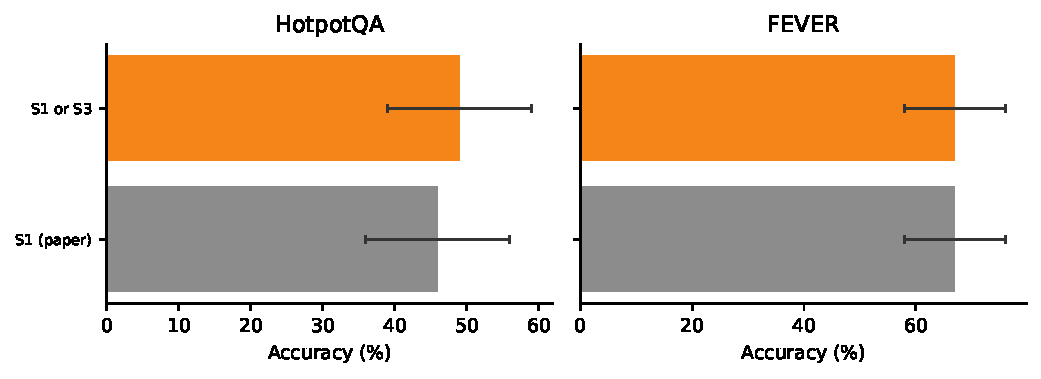
\includegraphics[width=\linewidth]{figures/fig_ablation.pdf}
\caption{Accuracy by trigger arm, ReAct$\to$CoT-SC, with bootstrap 95\% CIs.}
\label{fig:ablation}
\end{figure}

\begin{figure}[t]
\centering
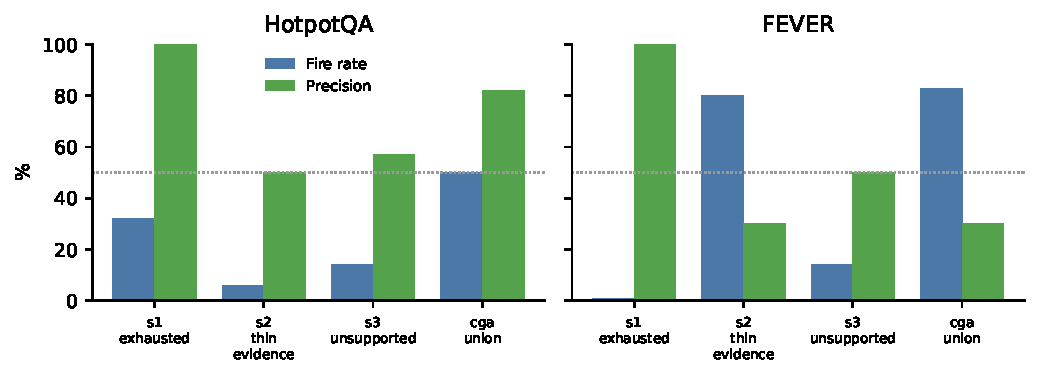
\includegraphics[width=\linewidth]{figures/fig_signals.pdf}
\caption{Per-signal fire rate vs.\ precision (diagnostic pass, $n{=}100$).}
\label{fig:signals}
\end{figure}

The direction is consistent: all four generalized-trigger comparisons in
Table~\ref{tab:ablation} move in the predicted direction (+1 to +3
percentage points), and none regresses. None reaches conventional
significance at $n{=}100$ --- the largest single-domain gap (HotpotQA
ReAct$\to$CoT-SC, +3pp) has only 5 discordant pairs total, which no
sample size below several hundred items could resolve at $p<0.05$. We
therefore do not claim a statistically confirmed accuracy improvement;
the study's stronger evidence is the signal-level precision-lift result
in Table~\ref{tab:signals}, which is a mechanistic claim (the trigger
fires on the right episodes) rather than an aggregate-accuracy claim, and
is not subject to the same discordant-pair sample-size limit.
